\chapter{Packages}
\label{package}

\go programs revolve around three principal constructs: rules, classes and packages -- in increasing order of granularity. In this chapter we focus on the larger scale aspects of \go programs -- namely \firstterm{package}{A package is a group of related definitions and programs that is separately compiled and loaded. Packages may contain classes, rules and types. Packages are accessed with the \q{import} statement.}s. Each \go source file makes up a package.

Packages represent \go's equivalent of modules; \go has a simple but effective package system that allows programs, classes and types to be defined in one file and re-used in others.

\index{Format of packages}
\index{Packages}
\index{Modules@\go packages}

Packages may contain type definitions, classes, rules, variables and constants. A top-level program also takes the form of a package -- with the addition of a standard action rule defined for the \q{main} symbol.

Packages may \q{import} other packages, in which case they are loaded automatically whenever the referring package is loaded. The \go engine guarantees that a given package will only ever be loaded once; although it does not necessarily guarantee the \emph{order} of loading, the system tries to ensure that packages are loaded in a way that dependent packages are loaded after the packages they depend on.

The form of a package source file is:
\begin{alltt}
\emph{packagename}\{
  \ldots
  \emph{Definitions}
  \ldots
\}
\end{alltt}
\index{Package names!file names of packages}
The \emph{packagename} is either a single identifier, or a sequence of identifiers separated by periods.

\index{package!name}
\index{name of package}
\index{files and packages}
Note that the \emph{packagename} must reflect the name of the file containing it. For example, if the package name is 
\begin{alltt}
foo.bar
\end{alltt}
then the \emph{name} of the file containing this package should be of the form:
\begin{alltt}
\ldots/foo/bar.go
\end{alltt}
i.e., the package source file must be located in a particular directory structure -- to the extent that the package name requires it.
\begin{aside}
The \emph{reason} for this is that the \go engine has to be able to locate the file containing the compiled package when it is loaded.
\end{aside}

\section{Package contents}
\label{package:contents}
\index{Contents of a package}

A package may contain class definitions, rule definitions, type definitions, package variable definitions, package constant definitions and initialization actions. It may also include directives to \q{import} other packages.

\index{Order of definitions}
\index{Packages!order of definitions in}
The order of definitions within a package is not important -- the \go compiler is able to handle mutually recursive programs without requiring forward declarations.

Many of the elements that may be found in a package are discussed elsewhere in this manual. In the following sections we focus on those elements that are not covered elsewhere.

\subsection{Package constants}
\label{package:constant}
\index{Constants in packages}
\index{Packages!constant in}

A package constant is declared at the top-level of a package, using a \q{=} statement:
\begin{alltt}
\emph{packageName}\{
  \ldots
  V:\emph{type}.
  V = \emph{initial}.
  \ldots
\}
\end{alltt}
The identifier \q{V} is constant in the sense that, once evaluated, it is not modifiable. It is evaluated as the enclosing package is loaded, in an order that is not guaranteed -- although the compiler attempts to ensure that any dependent values are evaluated before the variable itself is evaluated.

The type declaration for the variable is required; however, it can be folded into the statement thus:
\begin{alltt}
\emph{packageName}\{
  \ldots
  V:\emph{type} = \emph{initial}.
  \ldots
\}
\end{alltt}
Unlike package variables -- see Section~\vref{package:variable} -- package constants \emph{may} be exported from a package. In fact, by default, all allowable definitions in a package are exported. Thus constants declared in a package are made available to any packages that \q{import} the package.

\index{type inference!variable definition}
The type inference rule for a constant definition in a package is:
\begin{equation}
\AxiomC{\typeprd{E\sub{G}}{Ex}{T\sub{Ex}}}
\UnaryInfC{\extends{E\sub{G}}{\q{\emph{V} = \emph{Ex}},\mbox{E\sub{G}}}{(V,T\sub{Ex})}{\mbox{E\sub{G}}}}
\DisplayProof
\end{equation}
where \emph{E\sub{G}} is the environment derived from the package environment up to and including the definition of \emph{V} itself.

\begin{aside}
Package constants are evaluated in the full context of the package; i.e., the expressions that define their value can involve functions defined in the package and can even involve --directly or indirectly -- other package constants and variables.

However, if there is a circular dependency between package constants and variables; if the expression denoting the value of a constant refers to another constant, \emph{and} that constant's value expression also refers to this constant, then this can lead to serious problems when loading the package -- it is possible for the \go system to enter into a loop \emph{during the loading} of the module.

To try to prevent this, the compiler prints a warning message if it encounters what appears to be a circular dependency in package constants and variables.

This does not apply to mutually recursive programs however; as they are not evaluated as part of the package loading process. Therefore, it is quite safe to have mutually recursive programs. Furthermore, those mutually recursive programs may reference package variables and constants without harm.
\end{aside}


\subsection{Package variables}
\label{package:variable}
\index{Variables in packages}
\index{Packages!variables in}

A package variable is a re-assignable variable declared at the top-level of a package, using a \q{:=} statement:
\begin{alltt}
\emph{packageName}\{
  \ldots
  V:\emph{type} := \emph{initial}.
  \ldots
\}
\end{alltt}
Package variables have two major restrictions -- compared to regular logical variables -- their values must be ground at all times. In addition, variables are not exportable from packages. They also have a major freedom compared to logical variables -- they can be re-assigned.

If you need to export a package variable, then build accessor and mutator programs to manipulate the variable. For example, in
\begin{alltt}
mutator\{
  V : list[integer] := [].
  
  getV:[]=>list[integer].
  getV() => V.
  
  add2V:[integer]*.
  add2V(N) -> V := [N,..V].
\}
\end{alltt}
the variable \q{V} is not directly exported. The programs \q{getV} and \q{add2V} are exported; and can then be used by programs in other packages to modify \q{V}.

The merit of this approach is that the implementer of the \q{mutator} package is able to strictly control access to the variable -- making it simpler to be certain of the integrity of the variable's state.

\subsection{Package initialization}
\label{package:initialization}

In addition to package variables and constants having an initial expression associated with them, it is possible to define an action that will be executed on loading the package. Such initialization actions use the notation:
\begin{alltt}
\emph{packageName}\{
  \ldots
  \$ \{
    \emph{Action}
  \}
  \ldots
\}
\end{alltt}
The initialization action is executed \emph{after} any initializers associated with package constants and variables. Furthermore, if a package \q{imports} one or more other packages, then the initializers of those packages will also be run before the importing package's initializer -- thus ensuring that the initializer executes in a well defined environment.

A package can have any number of initializers in its body, however the relative order of execution between these different initializers is not defined.

Package initializers can be useful for certain classes of \emph{active} packages -- such as file system packages that may need to open certain standard files.

\subsection{Package exports}
\label{package:export}

By default, \emph{all} the exportable elements defined in a package are exported; except for re-assignable package variables. However, a definition may be prefixed by the \q{private} keyword, in which case the definition will not be exported.

The \q{private} keyword should appear before the first defining statement of the package element. For example, to define a \q{private} function \q{app}, the \q{private} keyword should be used as part of \q{app}'s type declaration:
\begin{alltt}
private app:[list[t],list[t]]=>list[t].
app([],X)=>X.
app([E,..X],Y)=>[E,..app(X,Y)].
\end{alltt}
\begin{aside}
This is a recommendation rather than a language restriction. The \go compiler will also pick up a \q{private} declaration if it precedes one of the rules that defines the program.
\end{aside}
The \q{private} keyword may be attached to program elements, constant declarations, class definitions or even type definitions.

\section{Importing packages}
\label{package:import}
\index{Importing packages}
\index{Packages!importing of}
\index{import@\q{import} directive}

The \q{import} directive in a package body is used to indicate that a particular package is required for that package. The form of the \q{import} statement is:
\begin{alltt}
import \emph{packagename}.
\end{alltt}
where \emph{packagename} is a dotted sequence of identifiers that matches the package name used in the package file. Note that \emph{packagename} must match exactly the package name used in the package's defining source file.

The effect of an \q{import} directive is to make available to the importing package all the definitions of the imported package. This includes classes, rules of various kinds, any types defined within the imported package and any \emph{constants} defined within the package.

The \go engine ensures that any given package will only be loaded once, however many requests for its \q{import} are found. Furthermore, any initialization code associated with a package (see \vref{package:initialization}) will also only be executed once.

\index{Circular chains of \q{import}s}
\index{Packages!recursive \q{import} not permitted}
\paragraph{Circular chains of \q{import}s}
The \go compiler requires that a package be compiled before it can be imported; more specifically the compiler searches for the compiled package when compiling a package that \q{import}s a package. Thus, it may be important to ensure that dependent packages are compiled after the packages that they depend on. It is not permitted to have a circular chain of package \q{import}s -- with one package importing another, which in turn causes the original to be imported.

It is possible for a package to \q{import} a package that \q{import}s other packages. These latter packages will be automatically loaded as needed. However, the definitions in these dependent packages are \emph{not} automatically made available to the original \q{import}er. For example, figure~\vref{program:packages:imports} illustrates a case with three packages: \q{foo}, \q{bar} and \q{jar}.
\begin{figure}
\begin{boxed}
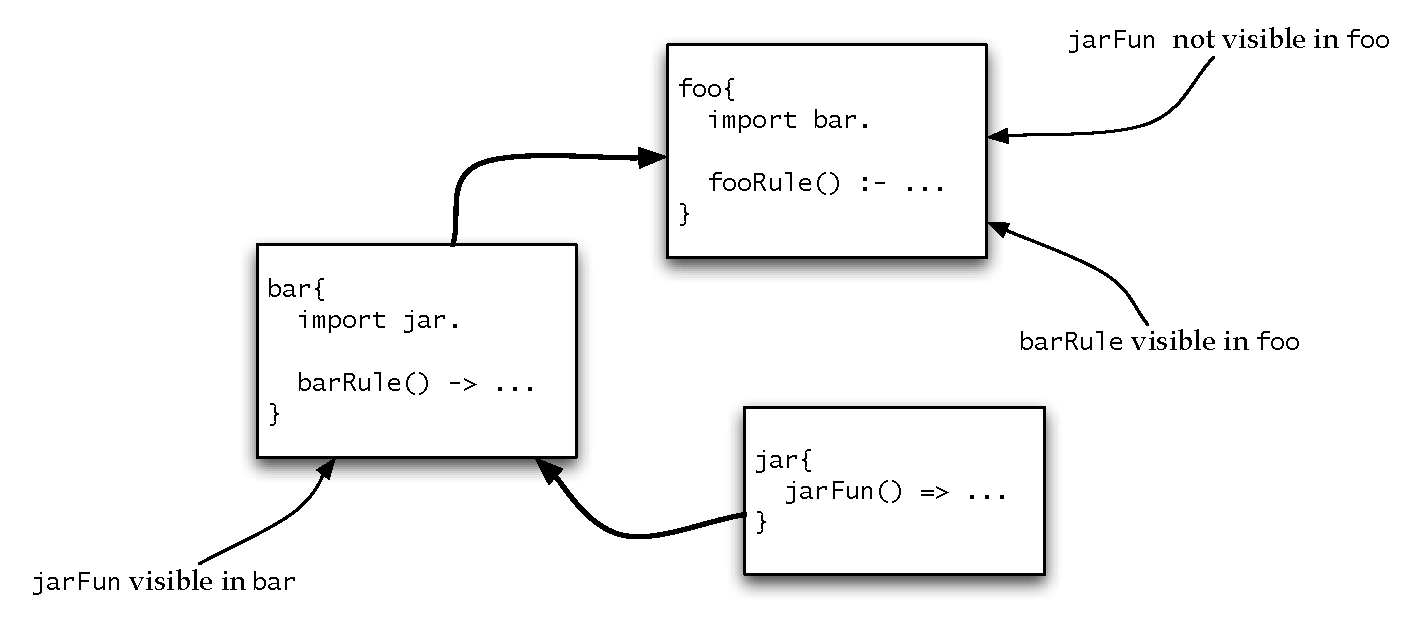
\includegraphics[width=\textwidth]{packages}
\end{boxed}
\caption{\label{program:packages:imports}A three-way package \q{import}}
\end{figure}
In this scenario \q{jarFun} is available within the \q{bar} package, but not in the \q{foo} package -- even though loading the \q{foo} package will cause \q{jar} to be loaded. If \q{jarFun} is required directly within the \q{foo} then it will have to be explicitly \q{import}ed by the \q{foo} package. Of course, the \q{barRule} action procedure is available within the \q{foo} package.

This can become an issue for type and other definitions that are shared over many packages. In that situation, the shared definitions will need to be \q{import}ed in each context that they are required.

\section{Top-level main programs}
\label{program:top-level}
Any package can also be treated as the top-level program -- provided that the package has a definition for the single argument action procedure \q{main}. In fact, \q{main} is a reserved word in \go: if a \q{main} program is defined in a package then it \emph{must} be consistent with the type assertion:
\begin{alltt}
main:[list[string]]*
\end{alltt}

If a package is executed at the top-level, then the \q{main} program in that package is executed and given as its single argument a list of the command-line arguments specified in the execution. For example, if a package \q{foo} were mentioned as the top-level package to execute in:
\begin{alltt}
\% go foo a b c
\end{alltt}
then the package \q{foo} must have an appropriate definition for \q{main} and that action procedure is entered -- with argument the list
\begin{alltt}["a","b","c"]\end{alltt}
\begin{aside}
Since the command line arguments are passed in as \q{string}s it is common for these argument strings to be parsed before they can be used in the application proper.  

The \q{\%\%} parse expression and the \q{go.stdparse} package become handy in this situation. For example, to pass a integer value to a \go fragment, where the number comes from the command line itself, then the classic way to do this is:
\begin{alltt}
mainPackage\{
  import go.stdparse.
  
  \ldots
  main([Arg,..More]) ->
    appProg(integerOf\%\%Arg);\ldots
\}
\end{alltt}
The \q{integerOf} grammar program parses a string into a \q{integer} value (see Section~\vref{stdparse:integerOf}).

See Chapter~\vref{compile} for further information on compiling and running \go programs.
\end{aside}

\section{Standard Packages}
\index{Packages!commonly loaded package}
Much of the functionality of the \go system is encapsulated in special packages that are not automatically included in every program. By convention, all \go system packages have package names of the form: \q{go.\emph{name}}; for example, the system input/output package is called \q{go.io}. To access the standard I/O package, then, it is necessary to load the \q{go.io} package:
\begin{alltt}
\emph{yourpackage}\{
  import go.io.
  
  \ldots
\}
\end{alltt}
\begin{aside}
The reason that \q{go.io} is not automatically included in every package is that that permits non-standard I/O systems to be used - for example in embedded applications, or in systems which have to interact with file systems in special ways.
\end{aside}
The standard set of packages will vary from time to time, the current set includes the packages
\begin{description}
\item[\q{go.cell}] Implements a re-assignable resource entity.
\item[\q{go.datelib}] Implements a collection of date related functions.
\item[\q{go.dynamic}] Implements dynamic relations; relations that can be updated.
\item[\q{go.hash}] Implements a hash-table package.
\item[\q{go.io}] Implements the standard I/O package
\item[\q{go.mbox}] Implements an internal thread communication package.
%\item[\q{go.scomms}] Implements a communication interface to the SCS.
\item[\q{go.setlib}] Implements a collection of set-like functions.
\item[\q{go.sort}] Implements a sort function
\item[\q{go.stack}] Implements a shareable updatable stack package.
\item[\q{go.queue}] Implements a shareable updatable queue package.
\item[\q{go.stdlib}] The standard \go language support package.\footnote{This package \emph{is automatically loaded} as it is required for successful execution of any \go program.}
\item[\q{go.stdparse}] Implements a range of parsing functions, allowing the conversion of strings to numbers, for example.
\item[\q{go.unit}] Implements a unit-testing framework.
\item[\q{go.xml}] Implements an XML parser and displayer package. Also defines the \go version of the DOM (Document Object Model).
\item[\q{go.http}] Implements many of the functions needed to build a Web server or an HTTP client.
\end{description}




